\section{Modelli SIMULINK utilizzati}
\label{app:SIMULINK}

	In questa appendice si riportano gli schemi \textit{SIMULINK} utilizzati, compresi dei relativi sottosistemi.

	\subsection{modello\_PID.slx}
	\label{subapp:modelloPID}
	
		Questa schema rappresenta la simulazione del motore elettrico CC controllato da un PID con desaturatore; lo schema del PID è riportato sotto.
		
		\begin{figure}[H]
			\centering
			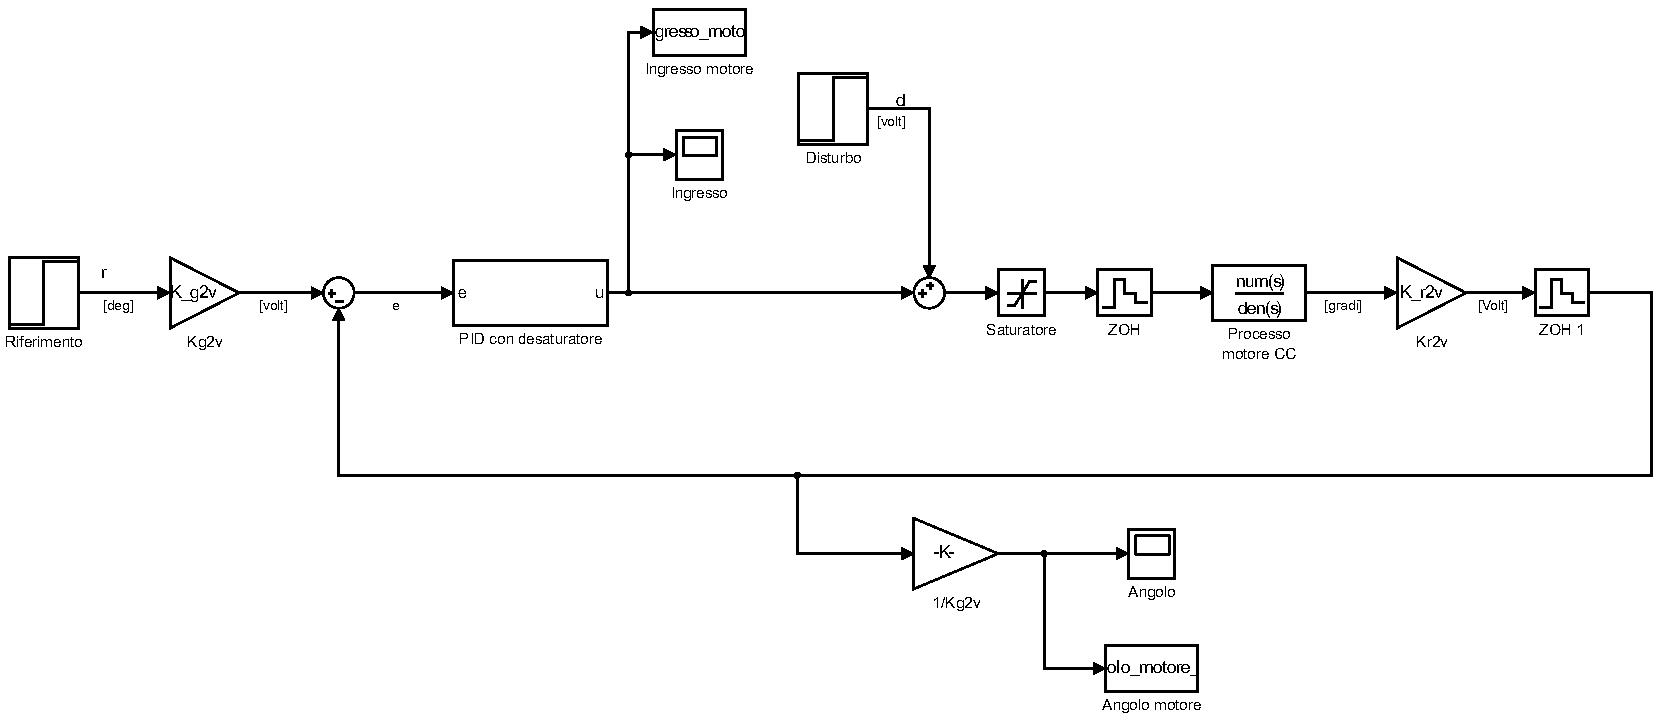
\includegraphics[scale=0.6]{./Figure/SIMULINK/modello_PID.pdf}
		\end{figure}
		
		\paragraph{PID con desaturatore}
		
			\begin{center}
				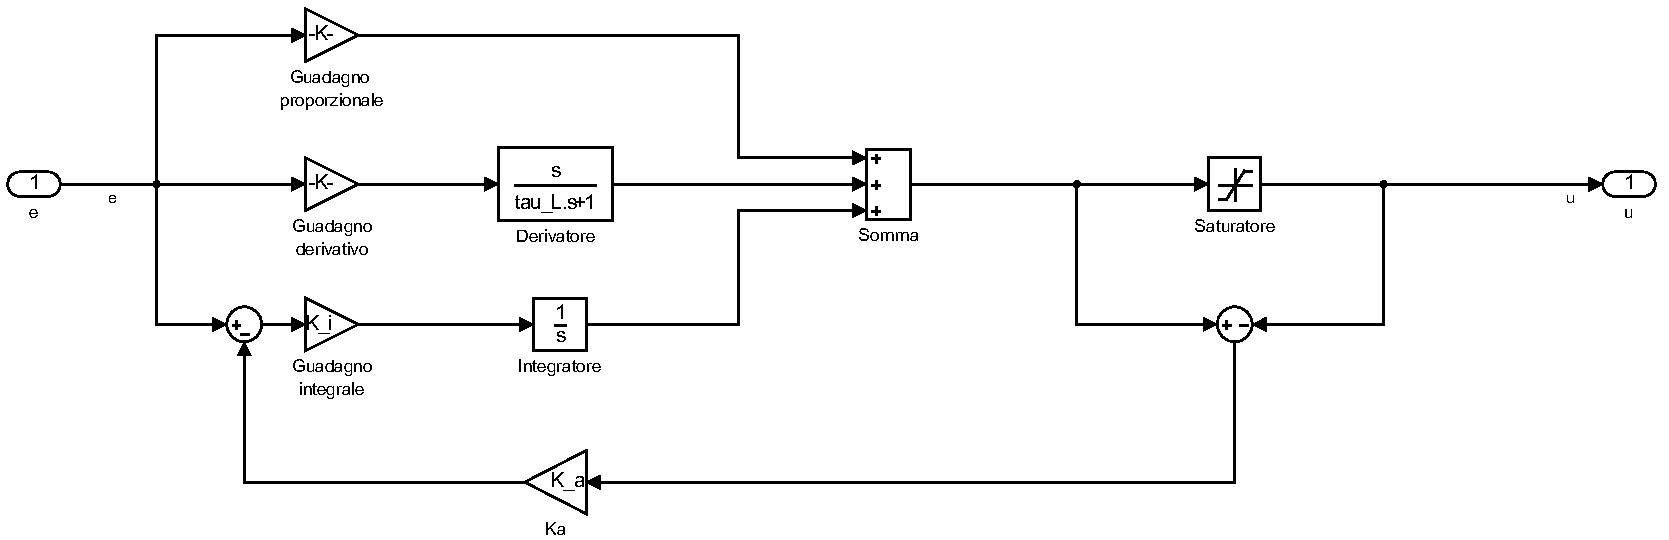
\includegraphics[scale=0.45]{./Figure/SIMULINK/PID_desaturatore.pdf}
			\end{center}
			
	\subsection{modello\_feedforward.slx}
	\label{subapp:modelloFF}
	
		\begin{figure}[H]
			\centering
			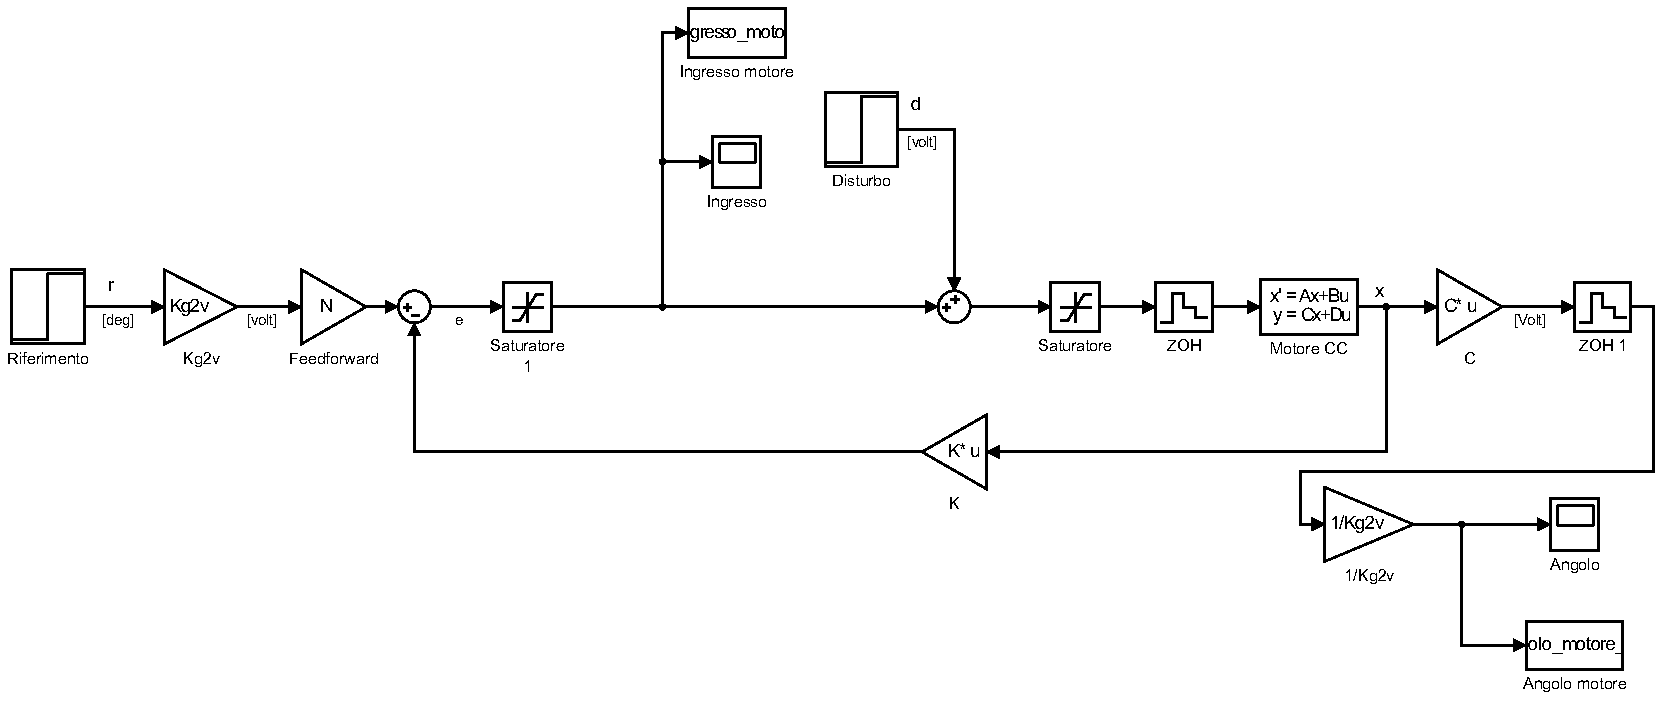
\includegraphics[scale=0.6]{./Figure/SIMULINK/modello_feedforward.pdf}
		\end{figure}			
		
	\subsection{modello\_integrale.slx}
	\label{subapp:modelloIntegrale}
	
		\begin{figure}[H]
			\centering
			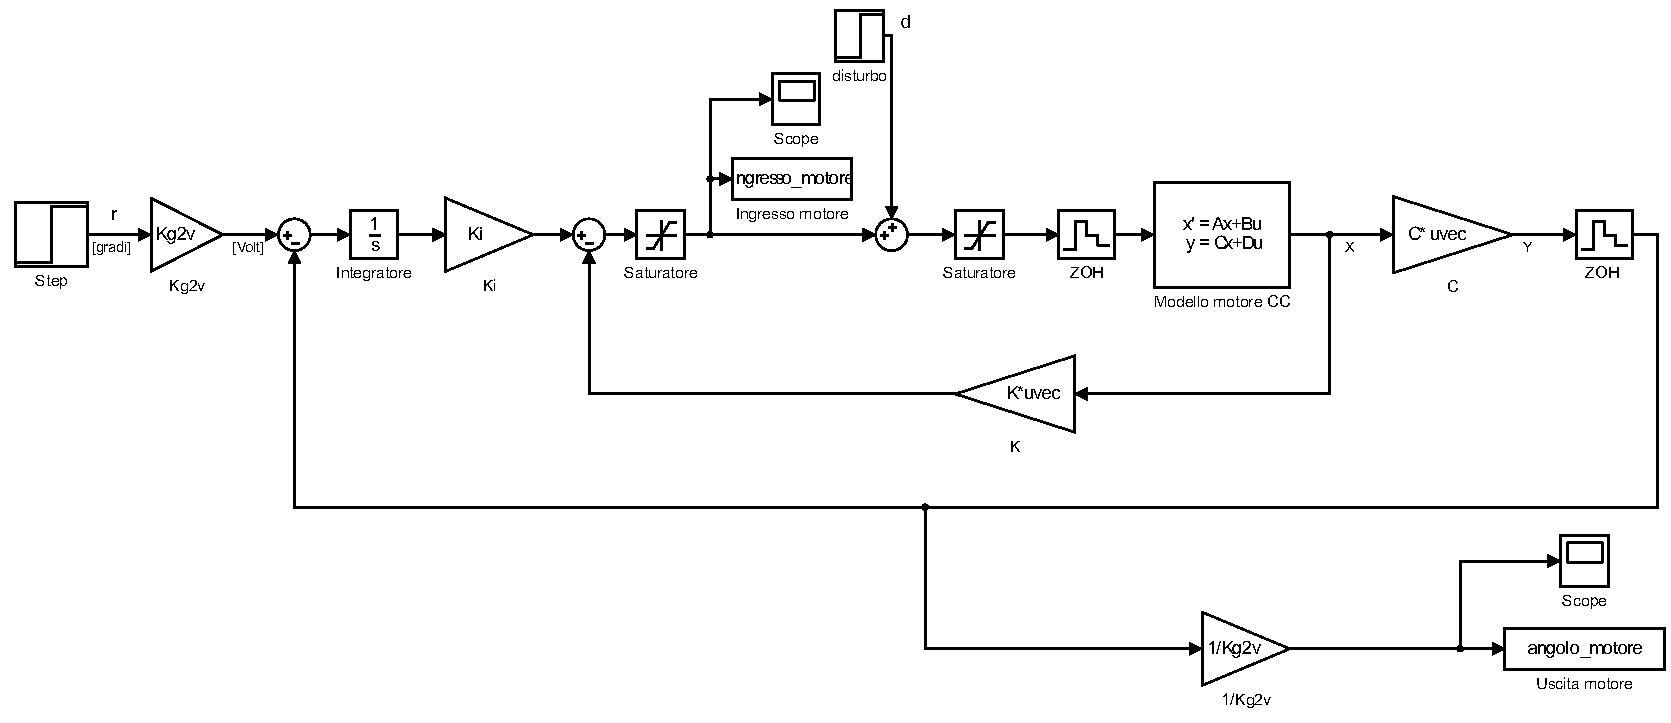
\includegraphics[scale=0.6]{./Figure/SIMULINK/modello_integrale.pdf}
		\end{figure}		
		